% This file is part of beamerthemepureminimalistic.

% If problems/bugs are found or enhancements are desired, please contact
% me over: https://github.com/kai-tub/latex-beamer-pure-minimalistic

\documentclass[a4paper]{book}
\include{version}
\usepackage{amsmath,amssymb,amsthm}
\newtheorem{thm}{Theorem}[section]
\newtheorem{theorem}{Theorem}[section]
\newtheorem{lem}[thm]{Lemma}
\newtheorem{lemma}[thm]{Lemma}
\newtheorem{prop}[thm]{Proposition}
\newtheorem{proposition}[thm]{Proposition}
\newtheorem{cor}[thm]{Corollary}
\newtheorem{corollary}[thm]{Corollary}
\theoremstyle{definition}
\newtheorem{Remi}[thm]{Reminder}
\newtheorem{rem}[thm]{Remark}
\newtheorem{defn}[thm]{Definition}
\newtheorem{ex}[thm]{Example}
\newtheorem{nonex}[thm]{{\bf NON}-Example}
\newtheorem{conj}[thm]{Conjecture}
\newtheorem{Exercise}[thm]{Exercise}
\newtheorem{Code}[thm]{Pseudocode}
\usepackage{datetime2}
\usepackage{graphicx}
\usepackage{svg}
% \svgpath{{/home/vassago/LATEX/}{/home/vassago/LATEX/svgs/}}
\usepackage{svg-extract}
\usepackage{hyperref}
\usepackage{inconsolata}

\usepackage{tcolorbox}

\usepackage[all]{xy}
\usepackage{xypic}
\usepackage{xcolor}

\definecolor{light}{RGB}{0,100,43}
\definecolor{dark}{RGB}{130,0,100}
\definecolor{exercise}{RGB}{220,200,255}
\definecolor{textcolor}{RGB}{0, 150, 128}
\definecolor{title}{RGB}{150, 0, 128}
\definecolor{footercolor}{RGB}{0, 128, 64}
\definecolor{code}{RGB}{240,220,160}
\definecolor{codebg}{RGB}{50,50,50}
\definecolor{mathbg}{RGB}{0,10,30}
\definecolor{mathtext}{RGB}{220,220,250}
\definecolor{bg}{RGB}{32, 0, 16}

\def\exercise#1{\color{light}{\h\Exercise{\color{exercise}\scshape #1}}\color{textcolor}}
\def\code#1#2{\color{dark}{\h\Code{\h}\\[.5em]%
\color{mathtext}#1
\begin{tcolorbox}[colback=codebg]%
\color{code}%
\texttt{#2}%
\color{textcolor}%
\end{tcolorbox}\color{textcolor}}}

\def\backtick{`}
\def\curtime{\DTMdate{2023-09-21} ~\DTMtime{01:42:17}\DTMdisplayzone{-5}{00}}
\def\light#1{{\color{light}#1}}
\def\dark#1{{\color{dark}#1}}
\def\h{\hspace{1em}}

\def\signature{\href{mailto:marc@lange-data.org}{Dr. Marc Lange, marc@lange-data.org}}
\def\mailsignature{\href{mailto:marc@lange-data.org}{marc@lange-data.org}}

\def\abs#1{\left| #1 \right| }
\def\floor#1{\lfloor #1 \rfloor }

\newcommand{\lthree}{<\hspace{-5.2pt}3}
\newcommand{\E}{\mathcal{E}}
\newcommand{\DAG}{\mathcal{DAG}}
\newcommand{\Z}{\mathbb{Z}}
\newcommand{\R}{\mathbb{R}}
\renewcommand{\P}{\mathfrak{P}}
\newcommand{\Q}{\mathbb{Q}}
\newcommand{\N}{\mathbb{N}}
\renewcommand{\S}{\mathbb{S}}
\newcommand{\C}{\mathcal{C}^{\leq}_{+} }
\newcommand{\D}{\mathbb{D}}
\newcommand{\LL}{\mathcal{L}^1(\Z,\Z)}
\newcommand{\Set}{\mathrm{Set}}

\renewcommand{\dag}{\mathrm{emb}\mathcal{DAG}}


\newcommand{\s}{Set^{\phantom{\leq}}_{\phantom{+}}}
\newcommand{\spp}{Set=fSet}
\newcommand{\smp}{Set^{\leq}_{\phantom{+}}}
\newcommand{\spm}{Set^{\phantom{\leq}}_{+}}
\newcommand{\smm}{Set^{\leq}_{+}}
\newcommand{\spmpm}{Set^{\pm}_{\pm}}

\newcommand{\App}{A}
\newcommand{\Amp}{A^{\leq}_{\phantom{+}}}
\newcommand{\Apm}{A^{\phantom{\leq}}_{+}}
\newcommand{\Amm}{A^{\leq}_{+}}

\begin{document}
\chapter{Restart DAGs 2024-03-05}
\section{Convenient Basics: Naturally Labelled Posets}
\defn[$NLPoset$]{
    The category of naturally labelled posets $\mathcal{N}$ has objects the following set:
    \[
    \begin{aligned}
    \mathcal{N}_0& =\\
    \{~(\lbrack n\rbrack,P)\in & \mathcal{P}_{fin}(\N)\times \mathcal{P}_{fin}(\N\times\N)~| \\ &~\lbrack n \rbrack = \{0,\ldots,n\}  \wedge P ~\mathrm{partial~~ order} \\ & \wedge P\subset \left( \leq_\N \cap ( \lbrack n \rbrack\times \lbrack n \rbrack ) \right) ~\}.
    \end{aligned}
    \]
    In words: Finite subsets $\{0,\ldots,n\}=:\lbrack n \rbrack \subset \N$ of the natural numbers with a partial order $P$, such that $\forall i \in \lbrack n \rbrack\colon iPi$, and $\forall i,j \in \N \setminus \lbrack n \rbrack\colon \neg ( iPj \vee jPi )$, and such
    that the poset order already implies naturally increasing labels $iPj \Rightarrow i\leq_\N j$. Write $(\lbrack n \rbrack, P)$ is an $NLPoset$ for this. In fact, $\lbrack n \rbrack$ is uniquely determined by $P$ as its diagonal $\lbrack n \rbrack = \{~ x\in\N ~|~ xPx ~\},$
    so we may choose to write only $P = (\lbrack n \rbrack, P)$, and set the (lexical) degree of P as $|P|:= \lbrack n \rbrack$.

    The morphisms are:
    \[
    \begin{aligned}
    \mathcal{N}_1 & = & \\
    & \{~ (P,Q,\varphi\colon |P|\rightarrow |Q|) ~| & \\
    P,Q\in \mathcal{N}_0 & \wedge \forall x,y \in |P| \colon xPy \Rightarrow \varphi(x)Q\varphi(y) ~\}. &
    \end{aligned}
    \]
    In words: The elements are pairs of posets with a monotonically non-decreasing map between them. Identities are monotonic, and composing set maps is associative, so this is a $(1-)$category.

    In particular the definitions of $\mathcal{N}_0$ and $\mathcal{N}_1$ exhibit the category easily as small, as in $\mathcal{N}_0$ describes only countably many objects, and since each of the
    objects $P,Q$ in the definition of $\mathcal{N}_1$ are themselves finite, there is only finitely many set maps $\varphi\colon |P|\rightarrow |Q|$ for each pair $(P,Q)$.
    So $\mathcal{N}_1$ is a countable union over finite sets, which are given by restricting source and target degrees $|P|, |Q|$ to a maximal degree. Hence $\mathcal{N}_0 \cup \mathcal{N}_1$ is
    a countable set, so $\mathcal{N}$ is an $\omega$-small $1-$category, if that means anything to the reader.
}

\section{Core Definition: The small Category of finite directed acyclic graphs.}
\defn[Category of DAGs]{
    In this text THE category of finite directed acyclic graphs $\DAG$, in short graph, is defined as follows.

    The objects are finite subsets of non-decreasing pairs of natural numbers including relevant diagonal elements:
    \[ \DAG_0 = \{~E\subset \N\times\N ~|~ \forall (x,y) \in E \colon x\leq y \wedge (x,x) \in E \wedge (y,y) \in E\wedge |E|<\infty ~\}. \]
    Say the edge set $E$ describes a directed graph $G(E)=(V,E)$. Call the edges of type $(x,x)$ vertices, i.e. "the vertex $x$".

    Morphisms are those maps of natural numbers that are monotonic with respect to the natural total order on natural numbers and respect these subsets:
    \[ \DAG_1(G_1,G_2) =\{~ \varphi \in \Set(\N,\N) ~|~ \forall (e_0,e_1) \in G_1 \colon (\varphi e_0, \varphi e_1)\in G_2 ~\}, \]
    Call the induced maps $\varphi_E\colon EG_1 \rightarrow EG_2$ and $\varphi_V\colon VG_1 \rightarrow VG_2$ for $VG=\{~x\in\N~|~(x,x)\in EG~\}.$
    Sometimes it is convenient to consider these morphism sets modulo the equivalence relation $\varphi \sim \psi :\Leftrightarrow \varphi_E = \psi_E \Leftrightarrow \varphi_V = \psi_V$,
    because clearly there is too much freedom in choosing a map $\N\rightarrow\N$ when the map is just supposed to be defined on a finite set.

    In particular morphisms are arranged just so that given our definition of objects,
    it is acceptable to collapse an edge $(x,y)$ onto a vertex with a map that
    satisfies $\varphi x = \varphi y$, but it is not acceptable to "break" an edge, i.e. map a pair of vertices that has an edge between
    in the source to a pair of vertices that does not.

    Call $\varphi\colon G \rightarrow H$ injective / surjective / bijective if the induced map on vertices $\varphi_V$ is injective/surjective/bijective.
}

\rem{
    Take extra care to note that the three properties injective, surjective, bijective exhibit massive difference in how they relate between
    vertices and edges.

    An injective map on vertices is clearly also injective as an map on the edge lists, trivially the converse is satisfied by including $(x,x)$ in the edge list.

    A surjective map on vertices however can fail maximally as follows:
    Set graphs
    \[ G_1 = \lbrack n\rbrack^\delta = \{(k,k)\}_{0\leq k \leq n}, G_2 = \Delta^{\lbrack n\rbrack} = \{ (i,j) \}_{0\leq i\leq j\leq n}. \]
    Then clearly the identity of $\N$ induces a natural map $G_1\rightarrow G_2$, which is surjective on vertices, but only on vertices not on edges, since
    $G_1$ does not have any edges $(i,j)$ with $i<j$.

    In particular bijectivity on vertices only implies injectivity on edges.
}

The following is a triviality, but an essential tool in this category.

\prop{
    Given two maps $\varphi,\psi\colon G\rightarrow H$ the maps are equal $\varphi=\psi$ if and only if they are so on vertices $\varphi_V=\psi_V$.
    \begin{proof}
    There is nothing to prove, the maps are defined as maps on vertices satisfying properties on edges.
    \end{proof}
}

\rem{
    Do notice that this definition still massively overrepresents even each isomorphism type of directed acyclic graph. The initial object, the
    empty graph represented by the empty subset of $\N\times\N$, is fortunately unique in this representation. The terminal object, the one-point
    graph however can be represented by any one-point set $\{(n,n)\}\subset \N\times \N$, so there are countably many isomorphic copies of those.

    However, it is evidently a small category: The objects are subsets of $\N\times\N$ with additional properties, hence countable.
    For the morphisms consider the full subcategories $G_n\subset \DAG$ of graphs with edge lists of length at most $n$, thus represent all morphisms
    of $\DAG$ with a union:
    \[ Mor\DAG = \bigcup_{n\in\N}\bigcup_{G\in G_n}\bigcup_{H\in G_n} \{G\}\times\{H\}\times\DAG(G,H). \]
    In particular the morphisms are a countable union of finite unions of finite sets, hence a countable set too.

    I shall make an effort to keep everything this small to keep it accessible to machine computation.
}

\prop{
    Every graph $G$ can be compressed isomorphically (usually non-uniquely) to an edge list with a minimal maximal vertex index in $\N$.
    \begin{proof}
    Let $G$ be a graph with edge list $EG$, which we can decompose as $EG = VG \sqcup \bar{E}G$ with
    \[
    VG := \{~x\in\N~|~(x,x)\in EG~\},~~ \bar{E}G := \{~(x,y)~|~x<y\wedge (x,y)\in EG~\}.
    \]

    Since $EG$ is finite, both those sets are too. In particular $VG \subset \N$ can be represented as a finite tuple of
    increasing natural numbers $(n_0,\ldots,n_k)$, hence define $\Phi\colon \N\rightarrow \N$ as
    \[ \Phi_{(n_0,\ldots,n_k)}(n):=\begin{cases}i &n\leq n_i\\ n & n>n_k\end{cases}. \]

    This map induces an order isomorphism $VG \cong \{0,\ldots,k\}$, hence define $\bar{G}$ with edge list $E\bar{G}:=\{ (i,j)\in \N\times\N | (n_i,n_j) \in EG \}$.

    Find that
    \[\Phi\colon G \rightarrow \bar{G} \]
    in fact induces an isomorphism of graphs, and $\bar{G}$ by construction could not be reduced in size to allow an injective map like that, so the maximal vertex
    of $\bar{G}$ is in fact the minimal possible maximal vertex of $\bar{G}$.


    \end{proof}
}

\ex{
    The complete graph on $n$ nodes or equivalently the $n$ simplex in a simplicial sense $\Delta^n$ can be represented as the object:
    \[ \Delta^n = \{~ (i,j) \in \N\times\N ~|~0\leq i\leq j\leq n ~\}. \]
    In particular each graph whose maximal vertex is $n$ can be embedded in such a $\Delta^n$, even uniquely given our model choices.

    The simplicially experienced would expect me to write down $\partial\Delta^n$ now, this is a bit more effort in this category with very stiff
    objects and morphisms, from $n\geq 2$ on one needs one subdivision step to represent $\partial\Delta^n$ as a dag.

    However, we can conveniently describe the horns:
    \[ \Lambda^n_k = \{~(i,j) \in \N\times\N~|~0\leq k\leq n \wedge ( (0\leq i\leq j \leq k) \vee (k\leq i \leq j \leq n))~\}, \]
    which have the evident inclusions:
    \[ j\colon \Lambda^n_k \rightarrow \Delta^n, \]
    given by the identity on vertices, and since the horn condition is stronger than the complete graph condition, this is a dag map.
}

\rem[Two specific Shuffles]{
    There are (far more than) two monotonic bijections:
    \[ \omega_\sqcup\colon \N\sqcup \N \rightarrow \N \]
    and
    \[ \omega_\pi \colon \N\times \N\rightarrow \N.\]

    A convenient description for $\omega_\sqcup$ can be given by embedding one copy of $\N$ as the odd numbers and one as the even ones. Write
    $(n,0)$ for elements from the first summand and $(n,1)$ from the second summand respectively. Then define a total order on $\N\sqcup \N$
    by $(n,i)\leq(m,i) \Leftrightarrow n\leq m$ in the same summand, $(n,0)\leq(m,1) \Leftrightarrow n\leq m$, and $(n,0)\geq(m,1) \Leftrightarrow n>m$.
    In particular the successor map on $\N\sqcup \N$ looks like a zig zag between the summands. Then $(n,i) \mapsto 2n+i$ is a order preserving
    bijection $\omega_\sqcup\colon (\N\sqcup \N,\leq_z) \rightarrow (\N,\leq)$, with inverse $\omega_\sqcup^{-1}( n ) = ( n//2, n \mod 2 )$.

    It is a bit more laborious to describe $\omega_\pi$. A typical diagram of the Hilbert hotel argument might go along the diagonals, e.g. $(0,2)\rightarrow(1,1)\rightarrow(2,0)$.
    However, for this application it is more convenient to go along boundaries of the square, like $(0,3)\rightarrow(1,3)\rightarrow(2,3)\rightarrow(3,3)\rightarrow(3,2)\rightarrow(3,1)\rightarrow(3,0)$.
    This yields a far nicer inverse formula based on a plain square root of natural square numbers.
}

\lemma{
    There is a bijection $\omega_\pi\colon \N\times\N \rightarrow \N$ given as:
    \[
    \omega_\pi(n,m):=\begin{cases} m(m+1)+n & n \leq m \\ n^2 +m & m \leq n-1 .\end{cases}
    \]
    In particular the cases describe the following image ranges explicitly:
    \[ \omega_\pi(\{0,\ldots,n\}\times\{n\}) = \{ n^2+n, \ldots, n^2+2n =(n+1)^2-1 \}, \]
    and
    \[ \omega_\pi(\{n\}\times\{0,\ldots,n-1\}) = \{ n^2, \ldots, n^2+n-1 \}. \]

    So find \[\N\times\N =\bigcup_{n\in\N} \{0,\ldots,n\}\times\{n\} \cup \{n\}\times\{0,\ldots,n-1\}, \]
    which maps to
    \[
    \begin{aligned}
    \omega_\pi(\N\times\N) & = \bigcup_{n\in\N} \{ n^2+n, \ldots, (n+1)^2-1 \} \cup \{ n^2, \ldots, n^2+n-1 \} \\
    & = \bigcup_{n\in\N} \{ n^2, \ldots, (n+1)^2-1 \} & = \N,
    \end{aligned}
    \]
    hence the map is surjective, and since that is true in each finite case $\{0,\ldots,n\}\times\{n\}$ and $\{n\}\times\{0,\ldots,n-1\}$ and
    the images are all disjoint, $\omega_\pi$ is injective too.
    \begin{proof}
    Note that both cases trivially satisfy either $\omega_\pi(n,m)=\omega_\pi(n-1,m)+1$ or $\omega_\pi(n,m)=\omega_\pi(n,m-1)+1$
    with a bit of magic for edge cases and the diagonal, so we can see the successor relation on the target $\N$ for most cases already. The reader is strongly encouraged to work out a few finite cases while
    staring at this lemma. It is trivial but confusing. I suggest "herringbone induction" as a name for this particular pattern.
    ~\\[5pt]
    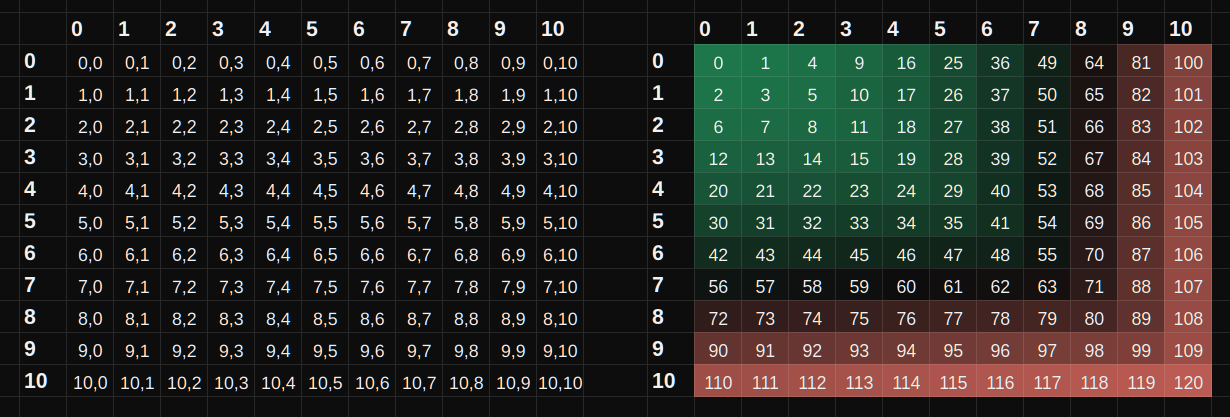
\includegraphics[width=0.75\textwidth]{omega_pi_sheet.png}\\[5pt]
    \end{proof}
}

\cor{
    There are the following recursion relations for columns and rows respectively:

    For $\varphi_n(m):=\omega_\pi(n,m)$ get:
    \[\varphi_n(m):=\begin{cases} n^2&m=0\\\varphi_n(m-1)+1&0<m<n\\\varphi_n(m-1) + 2(m+1) &n\geq m.\end{cases}\]

    For $\psi^m(n):=\omega_\pi(n,m)$ get:
    \[\psi^m(n):=\begin{cases} m^2+m&n=0\\\psi^m(n-1)+1&0<n\leq m\\\psi^m(n-1) + 2n+1 &n> m.\end{cases}\]

    In particular both grow linearly on a finite segment, and then quadratically into infinity.
}

\cor{
    The images of $\omega_\pi$ satisfy:
    \[ \omega_\pi(\{0,\ldots,N\}\times\{0,\ldots,N\})=\{0,\ldots,(N+1)^2-1\}. \]
}

\rem{
    I claimed the inverse formula for $\omega_\pi$ is nice, and I suspect some people might cringe at the appearance of
    floor as well as square root. For that: Try for any natural number $N$ you can conjure to approximate its $\floor{\sqrt N}$,
    you will find it is very easy to do by trying out natural squares in the vicinity until you're right. In other words: If you can
    memorise/understand $N$, you can definitely calculate $\floor{\sqrt N}$ and teach others to do it. E.g. for a relatively small
    example $99999$ is just one below $1000000 = 10^6$. The square root of $10^6$ is $10^3 = 1000$, hence, $\floor{\sqrt{99999}}=999$. }

I need a basic statement about natural squares and square roots.

\lemma{
    For all natural numbers there is the following relation between square and square root:
    \[ \forall N\in\N\colon \floor{\sqrt N}^2 \leq N < (\floor{\sqrt N}+1)^2. \]
    In particular
    \[ \forall N\in\N\colon   N \in \{\floor{\sqrt N}^2,\ldots, (\floor{\sqrt N}+1)^2-1\} \]
    \[ \Leftrightarrow \forall N\in\N\colon  N \]\[\in \{\floor{\sqrt N}^2,\ldots, \floor{\sqrt N}^2+\floor{\sqrt N}-1\}\sqcup \{\floor{\sqrt N}^2+\floor{\sqrt N},\ldots, (\floor{\sqrt N}+1)^2-1\}. \]
    \begin{proof}
    Since $(n+1)^2 - n^2 = n^2 + 2n + 1 - n^2 = 2n+1$, find that a natural number is either exactly a natural
    square or has an offset smaller than $2n+1$:
    \[
    \begin{aligned}
    &N = n^2+k&\wedge~~ &0\leq k < 2n+1 \exists! k,n\\
    \Leftrightarrow & \floor{\sqrt N} = n &\wedge~~& k = N-n^2 \in \{0,\ldots,n-1\}\sqcup\{n,\ldots,2n\}.
    \end{aligned}
    \]
    \end{proof}
}

\thm{
    There is an enumeration of pairs of naturals \[\varphi\colon \N \rightarrow \N\times\N,\]  which is inverse to $\omega_\pi$.
    \begin{proof}
    The core idea behind the formula was to make components recognisable by who contributed the square, so investigate that.

    For a natural number $N\in \N$ consider $k=\floor{\sqrt{N}}$, then by the lemma before find:
    \[ N - k^2 - k \in \lbrack -k, -1\rbrack \sqcup \lbrack 0, k\rbrack. \]

    So define:
    \[\varphi(N):=\begin{cases} (\floor{\sqrt{N}},N-\floor{\sqrt{N}}^2)
    & -\floor{\sqrt{N}} \leq N - \floor{\sqrt{N}}^2 - \floor{\sqrt{N}} < 0
    \\
    (N-\floor{\sqrt{N}}^2-\floor{\sqrt{N}},\floor{\sqrt{N}})
    & \floor{\sqrt{N}} \geq N - \floor{\sqrt{N}}^2 - \floor{\sqrt{N}} \geq 0.
    \end{cases}\]

    In particular the lemma implies that $\varphi$ is defined for each $N\in\N$.

    Since the results above already establish $\omega_\pi$ as a bijection, it suffices
    to show $\varphi\circ\omega_\pi = id_\N$, and by uniqueness of inverses for invertible
    maps it follows: $\omega_\pi\circ\varphi = id_{\N\times\N}$.

    Claim $\varphi\circ\omega_\pi = id_\N$, set $\omega_\pi(n,m)=N$ and $k=\floor{\sqrt{\omega_\pi(n,m)}}$
    as shorthands. Get
    \[
    \begin{aligned}
    \varphi(\omega_\pi(n,m))&=\begin{cases} \varphi(m(m+1)+n)& n\leq m\\ \varphi(n^2+m) & m<n. \end{cases}
    \end{aligned}
    \]
    Do recall that in the first case we get $\floor{\sqrt{m(m+1)+n}} = m$, while in the second case we get
    $\floor{\sqrt{n^2+m}}=n$. In particular in the first case $N-m^2-m = n$, in the second case $N-n^2=m$.
    Note additionally that the cases of $\varphi$ are arranged just so that they correspond to the cases
    of $\omega_\pi$, i.e. for $n\leq m$ get: $N - \floor{\sqrt{m(m+1)+n}}^2-\floor{\sqrt{m(m+1)+n}} = N-m^2-m=n \geq 0$,
    so this is covered by the second case of $\varphi$. For $n>m$ get: $N-n^2-n = m-n < 0$, hence the first case
    of $\varphi$ applies.
    \[
    \begin{aligned}
    \varphi(\omega_\pi(n,m))&
    =\begin{cases}
     (N-m^2-m,m) & n\leq m \\
     (n, N-n^2) & m<n .
    \end{cases}\\
    &=\begin{cases}
     (n,m) & n\leq m \\
     (n,m) & m<n .
    \end{cases}&=(n,m).\\
    \end{aligned}
    \]
    Since $\omega_\pi$ has already been established as invertible, get $\omega_\pi(\varphi(N))=N ~\forall N$, too.
    \end{proof}
}

\rem{
    Do note that $\omega_\sqcup$ and $\omega_\pi$ each are not associative, in the sense that threefold sums or
    products have different results depending on which two factors / summands are combined first.

    Consider the threefold sum $\N\sqcup\N\sqcup\N$ and a number in the middle summand, then get
    \[ (\omega_\sqcup\circ (id\times\omega_\sqcup))(n,1) = \omega_\sqcup(2n,1) = 2*2n+1, \]
    but
    \[ (\omega_\sqcup\circ (\omega_\sqcup\times id))(n,1) = \omega_\sqcup(2n+1,1) = 2*(2n+1)+1 = 4n+3. \]
    So, for example the zero of the middle summand is sent to $1$ by the upper combination and
    sent to $3$ by the lower combination.

    Similarly for $\N\times\N\times\N$ consider any tuple $(k,l,m)$ with $k>l^2+m>l>m$ and e.g. $k^2+l>m$, get
    \[ (\omega_\pi\circ (id\times\omega_\pi))(k,l,m) = \omega_\pi(k,l^2+m) = k^2+l^2+m , \]
    but
    \[ (\omega_\pi\circ (\omega_\pi\times id))(k,l,m) = \omega_\pi(k^2+l,m) = (k^2+l)^2+m . \]
    So e.g. $(1,2,1)$ maps to $1+4+1=6$ above, while it maps to $(1+2)^2+1=10$ below.

    Both maps have been chosen to suppress "for graphs with vertex counts $g,h$" and sentences like that from
    what follows, with more care about degrees, associativity like this can be achieved.
}

TODO: hiermit, graph internal to discrete dags!? das sollte n diskretisierungsschritt sein :)

TODO: n graph mit crig weighted edges (aber 1 auf den knoten) ist ne SL matrix $\rightarrow$ multiplizieren, kategorie, gedoens
sub-TODO: was passiert wenn $(x,y)\in G \Leftrightarrow w(x,y) \neq 0?$

\lemma[$\DAG$ has sums]{
 Let $G = \{~ (x_k,y_k)~|~k\in\{0,\ldots,|E(G)|\} ~\}$ and $H = \{~ (x_k,y_k)~|~k\in\{0,\ldots,|E(H)|\} ~\}$ be
 two finite dags represented as edge lists with pairs of natural numbers representing the edges.

 Define the sum of $G$ and $H$ as the edge list
 \[G\sqcup H = \{~ (2n,2m) ~|~ (n,m)\in E(G) ~\}\sqcup\{~ (2n+1,2m+1) ~|~ (n,m)\in E(H) ~\}.\]

Thus there exist graph inclusions $G\rightarrow G\sqcup H$ and $H\rightarrow G\sqcup H$ given by
sending $G$'s coordinates to their doubles and $H$'s coordinates to their doubles plus one.

In addition the universal property holds, i.e. for each other graph $Z$ and each pair of morphisms
with that target $G\rightarrow Z$, $H\rightarrow Z$, there exists a unique map $G\sqcup H \rightarrow Z$,
compatible with the given maps and inclusions.

\begin{proof}
The most essential insight is that the zig-zag ordering on the sum $\N\sqcup\N$ makes the identification
via $\omega_\sqcup$ order-preserving between two total orders. Hence the edges that appeared as $(n,m)$
in either $G$ or $H$, hence satisfy $n\leq m$, satisfy $2n\leq 2m$ and $2n+1\leq2m+1$, so are compatible
with the vertex embedding of $G\sqcup H$.
\end{proof}
}

\lemma[$\DAG$ has products]{
    Given two graphs $G,H$ with $G = \{~ (x_k,y_k)~|~k\in\{0,\ldots,|E(G)|\} ~\}$ and $H = \{~ (x_k,y_k)~|~k\in\{0,\ldots,|E(H)|\} ~\}$ represented as edge lists with pairs of natural numbers representing the edges.

    Define the product of $G$ and $H$ as the edge list:
    \[G\times H =\{~(\omega_\pi(k,l),\omega_\pi(m,n))~|~(k,m)\in G\wedge (l,n) \in H~\}.\]

    Do note how the detail features that $(x,x)$ edges are included in our definition of dags, in that
    these edges contribute a lot of product edges.

    Then there exist dag morphisms $G\times H \rightarrow G$ and $G\times H \rightarrow H$, the canonical projections,
    with the universal property of the product: For each source graph $X$ and pair of morphisms
    $X\rightarrow G$, $X\rightarrow H$
    there exists a unique dag morphism $X\rightarrow G\times H$ compatible with the given pair of morphisms and
    the canonical projections.
    \begin{proof}
    The row wise and columnwise inductions for $\omega_\pi$ do show that both are strictly monotonic for each
    row and column, in particular $\omega_\pi$ is monotonic for the product order on $\N\times\N$ with
    $(a,b)\leq(c,d) :\Leftrightarrow a\leq c \wedge b\leq d$. So find that $(k,m)\in G$ and $(l,n)\in H$ imply
    $k\leq m$ and $l\leq n$, hence $(k,l)\leq (m,n)$, so $(\omega_\pi(k,l),\omega_\pi(m,n))$ is a legal edge, as it is non-decreasing.
b    \end{proof}
}

\section{Constructions on DAGs}
\defn{
    sum
}
\defn{
    initial object
}
\defn{
    pushouts
}
\defn{
    product
}
\defn{
    terminal object
}
\defn{
    pullbacks
}

\defn{
    flags!
}

\subsection{Functorial Factorisation}
Each graph $G$ can be embedded in a unique graph $\Delta G=\coprod_i \Delta^{n_i}$ (nicht ganz, nur wenn verschiedene urbilder nicht verbunden sind).

\section{The Core Construction: Subdivision}
TODO: hier ist harter off-by-one trouble drin .. fuegt Sd n basispunkt hinzu? sollte ich alles punktieren?
\lemma[The Power Set Map]{
    For $P_{fin}(\N) = \{~ S\subset \N ~|~ |S|<\infty~\}$ the finite subsets of natural numbers we can define a map:
    \[ b\colon P_{fin}(\N) \rightarrow \N \]
    by assigning to a finite set its binary encoding:
    \[ \{n_0,n_1,\ldots,n_k\} \mapsto \sum_{0\leq i \leq k} 2^{n_i} ( - 1 ? ). \]
    It is evidently injective, one can recover each $n_i$ as the binary digit indices where there is a $1$. It is also surjective, each
    natural number can be written as a finite binary word. Call the inverse $\pi\colon \N \rightarrow P_{fin}(\N)$, after all its target
    is the power set of its domain :) So for each $n\in \N$ we have a unique corresponding finite subset $\pi(n) \in P_{fin}(\N)$.
    The map has another very pleasant property, it is monotonic. Specifically, a proper subset inclusion corresponds to adding
    $1$s in the binary representation, so the number increases.
}

\defn[Subdivision of DAGs]{
    Let $E(G) \subset \N \times \N$ describe a directed graph $G$.

    Define the edge set
    \[E(Sd(G)) = \{~ (n,m) =(\sum_{i} 2^{s_i}, \sum_{j} 2^{t_j})  ~|~  \] \[ \{s_i\}_i\subset\{t_j\}_j \forall i,j\colon (s_i,t_j) \in E(G) \wedge (s_i,s_j)\in E(G) \wedge (t_i,t_j)\in E(G) ~\}.\]
    In words: The vertices are the numbers $n = \sum_i 2^{s_i}$ such that each non-decreasing pair $(s_i,s_j)$ is an edge in $E(G)$, call those legal vertices.
    Between each such pair of legal vertices $n=\sum_i 2^{s_i},m=\sum_{j} 2^{t_j})$, set $S=\{s_i\}_i,T=\{t_j\}_j$. Add an edge $(n,m)$ if and only if $S\subset T$.
}

\rem{
    Do note that since $S\subset T$ is an inclusion of legal vertices, each "new" edge has already been "tested" by $T$.
}

\ex[Subdivision of $\Delta^n$]{
    Recall $\Delta^n$ is represented by the edge set $\{(i,j)|0\leq i \leq j \leq n\}$.
}

TODO: erlaubte quotienten ... $\Delta^n$ zweimal subdividen und dann rand weg ist erlaubt und gibt $\S^n$.

TODO: schwache aequivalenzen sind hin und rueck kompositionen von acyclic cofibrations und acyclic fibrations.. also blow-up und collapse

\section{Cofibrations, Fibrations, Weak Equivalences, Homotopy, Connected Components, Factorisations, Cell Structures}

\[I:=\{n^\delta \rightarrow \Delta^n\}_{n\in\N}\]
und mit $P^n = \{~(i,i+1)~|~0\leq i < n~\}$, i.e. $P^1 = ( \bullet \rightarrow \bullet ), P^2 = ( \bullet \rightarrow \bullet \rightarrow \bullet )$
\[J:=\{P^n \rightarrow \Delta^n\}_{n\in\N}\]

Clearly $I-cell$ are exactly the injective maps, if there is an injection on vertices, there is one on edges, so count the edges,
and sum over them.

pushouts fuer vertex injektiv!?

w.eq's, abb'n $f\colon X\rightarrow Y$ such that $\exists g\colon U \rightarrow V$ and acyclic cofibrations (circular, vorsicht)



\end{document}
